% ----- APPENDIX I ------------------%
%                                    %
%      The Peanuts                   %
% ---------------------------------- %
\chapter{Antenna Response}
\label{app:peanut}

%\begin{figure}[!h]
%\centerline{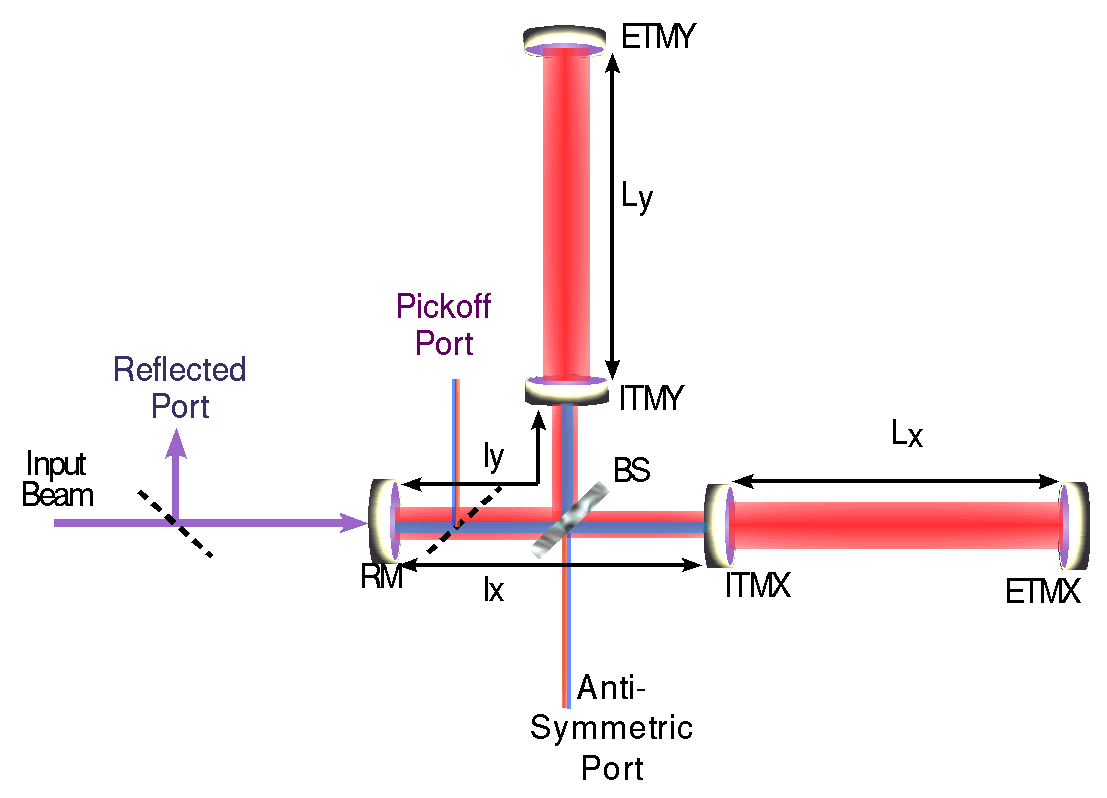
\includegraphics[angle=0,width=6.5in]{Figures/Chap3/IFO2.png}}
%\end{figure}

An important consideration to make in evaluating the sensitivity of any
detector is its directional response. The directional antenna response of
an interferometer is derived in \cite{Sigg:GW} and \cite{Nelson:Thesis}.

From Equation~\ref{eq:hmatrix} we have the form for the strain perturbation
tensor in the detector's coordinate system for a wave incident on the detector
from the positive z-direction. The strain along the interferometer arms
for a source from an arbitrary direction is
\begin{equation}
h_{xx} = - \cos(\theta) \sin(2 \phi) h_{\times} +
          (\cos^2(\theta) \cos{\phi}^2 - \sin{\phi}^2) h_{+}
\end{equation}

\begin{equation}
h_{yy} =  \cos{\theta} \sin{2 \phi} h_{\times} +
          (\cos{\theta}^2 \sin{\phi}^2 - \cos{\phi}^2) h_{+}
\end{equation}
The antenna response at DC is propotional to $|h_{yy}-h_{xx}|$. The next three
plots show this DC response for $+$ waves, for $\times$ waves, and for unpolarized
waves (quadrature sum of the two cases). In the coordinate system used in these
plots, the interferometer is located at the origin with the arms parallel to the
x and y axes.


\begin{figure}[!h]
\centerline{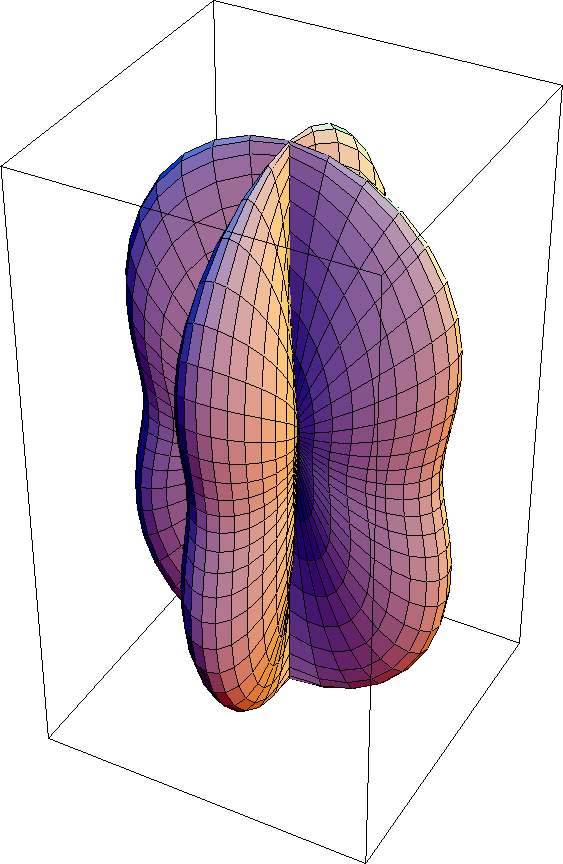
\includegraphics[angle=0,height=7.5in]{Figures/AppI/Peanut-plus.png}}
\caption[Peanut (plus)]{Antenna response for the $+$ polarization.}
\label{eq:Peanut-plus}
\end{figure}

\begin{figure}[!h]
\centerline{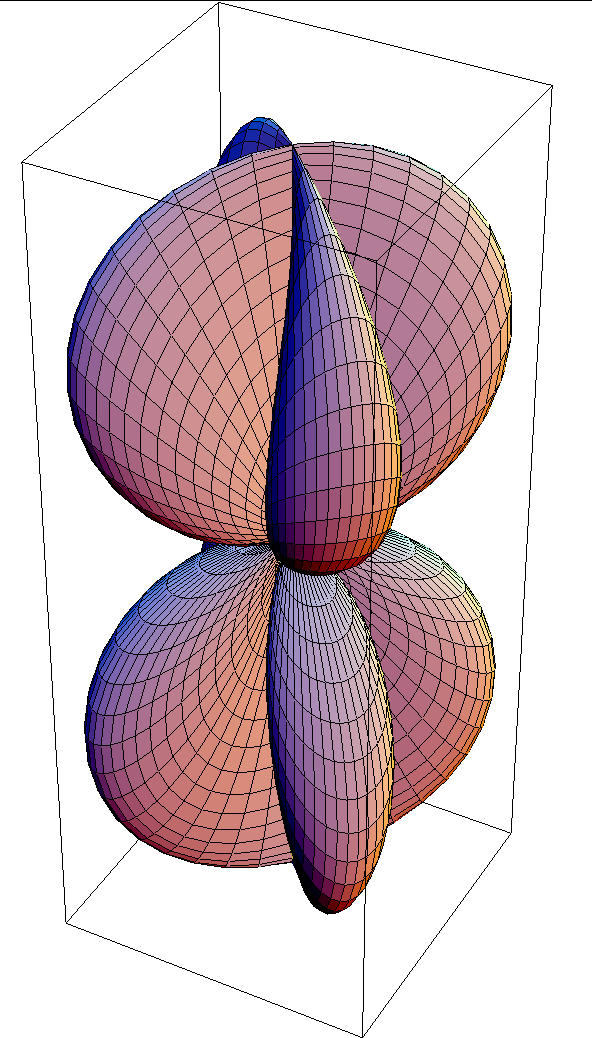
\includegraphics[angle=0,height=7.5in]{Figures/AppI/Peanut-cross.png}}
\caption[Peanut (cross)]{Antenna response for the $\times$ polarization.}
\label{eq:Peanut-cross}
\end{figure}

\begin{figure}[!h]
\centerline{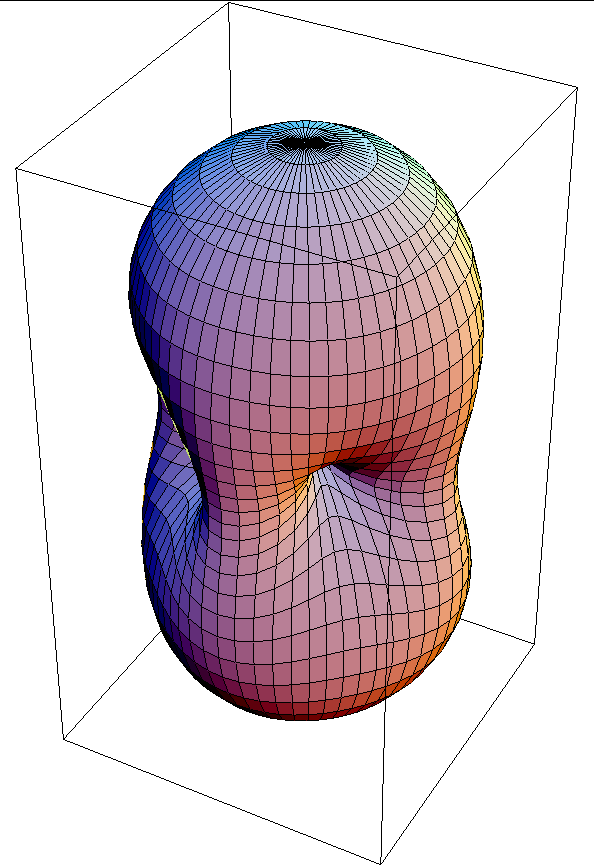
\includegraphics[angle=0,height=7.5in]{Figures/AppI/Peanut-unpol.png}}
\caption[Peanut (un-polarized)]{Antenna response for the unpolarized waves. 
         This is plotted as just the quadrature sum of the $+$ and $\times$ waves.}
\label{eq:Peanut-unpol}
\end{figure}







